\section{Vortex formation at planetary gap edges in layered
  discs}\label{disc-planet} 
The previous simulations, while necessary to isolate the effect of 
viscosity on the linear RWI, has the disadvantage that the radially
structured viscosity profile may act to source radial disc structure
in the non-linear regime. In this section, we use disc-planet interaction to
create the disc structure required for instability, and employ a radially smooth
viscosity profile. We therefore expect viscosity to only
act as a damping mechanism. 

Vortex formation at gap edges is seen in many  
2D and 3D hydrdynamical simulations of giant planets in low viscosity discs 
\citep{valborro07,lin10,lin11a,lin12}. The fact that this is due to
the RWI has been explicitly verified through linear stability
analysis of planetary gap profiles produced from 2D simulations
\citep{valborro07,lin10}. Here, we simulate gap-opening giant planets
in 3D discs where the kinematic viscosity varies with height above the
disc midplane. Our numerical experiments are similar in spirit to
those performed by \cite{pierens10}, but our focus here is gap
stability in a layered disc. 
 
\subsection{Radially smooth viscosity profile for disc-planet
  interaction}\label{planet_visc_mode} 
Using the same notation as \S\ref{visc_model}, we impose a viscosity
profile $\hat{\nu}$ such that 
\begin{align}\label{planet_visc_profile}
  \hat{\nu}\Sigma_i(R)=%\frac{d\ln{\Omega_i}}{d\ln{R}} =
  \hat{\nu}_0\left[1+Q(\psi)\right]\Sigma_i(r_0)%\left.\frac{d\ln{\Omega_i}}{d\ln{R}}\right|_{r_0}.      
\end{align}
We have set the dimensionless argument in Eq. \ref{step} to
$\zeta=\psi$. Recall $\psi=\pi/2-\theta$ is the angular height away from the midplane. 
The viscosity increases from its floor value $\hat{\nu}_0$ by a factor
$A_\nu$ for $\psi > \zeta_\nu$. So the viscous layer is 
a wedge in the meridional plane, which conveniently fits into our
spherical grid. %Note that setting $\psi = 0$ in Eq. \ref{planet_visc_profile} gives
%the appropriate viscosity profile for a razor-thin viscous disc in
%steady state when the initial cylindrical radial velocity 
%is set by Eq. \ref{init_vr}. 

The typical viscosity value adopted for disc-planet simulations, 
$\hat{\nu}\sim 10^{-5}$ or $\alpha\sim 10^{-3}$, is known to surpress
vortex formation in 2D \citep{valborro07, mudryk09}. 
We therefore choose a floor viscosity of $\hat{\nu}_0=10^{-6}$.
The angluar thickness of the viscosity transition is fixed to
$\Delta\zeta_\nu = 0.2h$. Fig. \ref{planet_visc2d} gives an example of this
viscosity profile. We will quote the thickness of the viscous layer as a 
percentage of the entire $\theta$ domain size. 

\begin{figure}
  \centering
  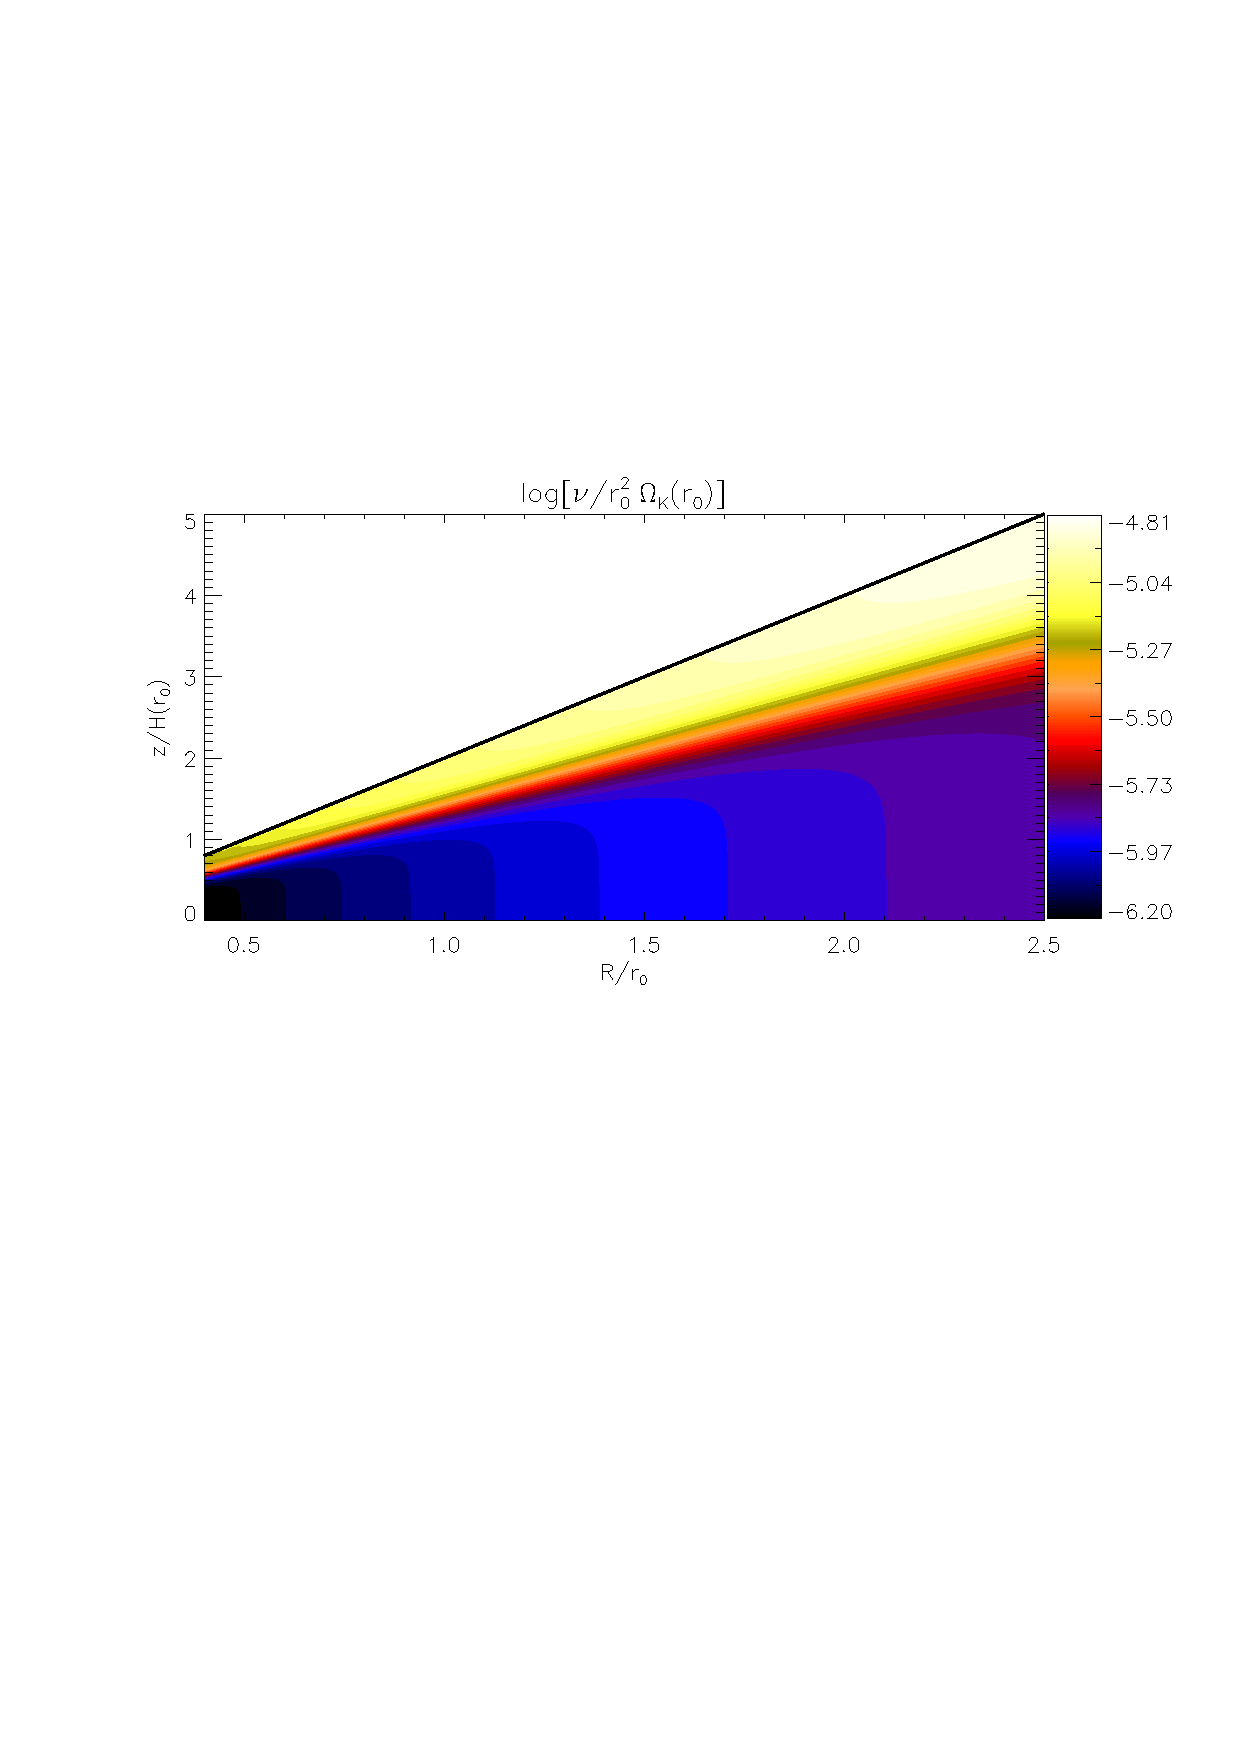
\includegraphics[width=\linewidth]{figures/pdisk_visc2d_planet}
  \caption{Example of the `wedge' viscosity profile
    imposed in disc-planet simulations
    (Eq. \ref{planet_visc_profile}).  
    For a disc with constant aspect ratio, as chosen here, the viscous
    layer occupies a constant number of scale heights across the
    radial range. This specific plot corresponds to case P1, so the
    viscous layer (yellow-white colours) always occupies the uppermost
    $H$ at each cylindrical radius. 
    The solid line
    delineates the upper boundary of the computational domain.
    \label{planet_visc2d}}
\end{figure}

%This viscosity profile is a smooth
%function of radius, meaning a localized radial density structure will
%be smoothed out, unless it is maintained by an external
%source (the planet in our case). We therefore expect viscosity to only
%act as a damping mechanism, c.f. a source for radial structure in the
%previous section. 

\subsection{Disc-planet simulations} 
We simulate locally isothermal discs with constant aspect-ratio
$h=0.05$ (by choosing $q=1$), vertical extent $n_h=3$ scale-heights 
and radial extent $[\rin,\rout]=[0.4,2.5]r_0$. Initially the surface density is smooth
($A=1$) with zero meridional velocity ($v_r=v_\theta=0$). 
%cylindrical radial velocity is given by
%Eq. \ref{init_vr}. 
The standard resolution is $(N_r, N_\theta,
N_\phi)=(256, 32n_h, 768)$, corresponding to $6,\,32,\,6$ 
cells per $H$ along the $r,\theta,\phi$ directions at the reference
radius. We apply a damping rate $\hat{\gamma}=2$ with the reference
velocity field $\bm{v}_\mathrm{ref}=(0,0,v_\phi)$ in spherical
co-ordinates.   

We insert into the disc a planet of mass  
$M_p=10^{-3}M_*$, which corresponds to a Jupiter mass planet if
$M_*=M_{\sun}$. The softening length adopted for the planet potential is
$\epsilon_p=0.5r_h$. The planet potential is switched on 
smoothly over $t\in[0,10]P_0$. We note that the disc can be considered
as two-dimensional for gap-opening giant planets, because the Hill
radius $r_h$ exceeds the local scale-height $H_0$ ($r_h/H_0\simeq1.4$
in our cases).   

We remark that the above choice of physical and numerical parameter
values are typical for global disc-planet simulations
\citep[e.g.][]{valborro06,mignone12}.   

%\subsubsection{Standard runs} 
%The fiducial vertical extent of our disc model is $n_h=2$
%scale-heights at $R=r_0$.  The control run, case P0, has $A_\nu=1$ so there is 
%no viscous layer. The kinematic viscosity is therefore
%$\hat{\nu}\sim10^{-6}$  everywhere. We then introduce a viscous
%layer (or wedge) occupying the uppermost $25\%$ and $50\%$ of the
%vertical domain in cases P1 and P2, by choosing the transition angle
%at $\zeta_\nu = 1.5h,\,1.0h$, respectively. These layers have a kinematic 
%viscosity of $\hat{\nu}\sim 10^{-5}$ by setting $A_\nu=10$.  (See
%Fig. \ref{planet_visc2d} for the viscosity profile for case P1.)  


\subsubsection{Runs}
%We also consider two runs with an extended vertical domain size
%$n_h=3$. 

Our fiducial case P0 has $A_\nu=1$ so there is no viscous layer, thus
$\hat{\nu}\sim 10^{-6}$ everywhere. For case
P1 and P2 we set $A_\nu=100$ with transition angle $\zeta_\nu=2h$ and
$h$, respectively. Thus the viscous layer with $\hat{\nu}\sim10^{-4}$
occupies the upper $H$ and $2H$ of the vertical domain. We also
consider case P0.5, in which we resume case P0 from 
$t=100P_0$ but with the layered viscosity profile of case P1. 

%Thus, the viscous layer with $\hat{\nu}\sim10^{-4}$ occupies $33\%$ of
%the uppermost vertical domain. %Note that most of the mass is contained
%in the low viscosity layer. 
%We also consider case P6 without a
%viscous layer but 


%%%%%%%%%%%%%%%%%%%%%%%%%%%%%%%%%%%%%%%%%%%%%%%%%%%%%%%%%%%%%%%%%%%%%%%%%%%%%%%


\subsection{Results}
Our disc-planet simulations are summarised in Table \ref{planet_sims}.
We focus on vortex-formation at the outer gap edge. 
The non-axisymmetric mode amplitude in the last column was 
averaged over the shell $r\in[1.2,1.6]r_0$ and over time 
$t\in[100,150]P_0$. We examine the $m=1$ mode since 
for non-self-gravitating planetary gaps, if unstable, usually develop
a single vortex in quasi-steady state \citep{valborro07,lin10}.   

%for  mode amp: spatial average over [1.2,1.6], time average over [100,150]P_0

\begin{table}
  \centering
  \caption{Summary of disc-planet simulations. These runs employ the
    `wedge' viscosity model described by
    Eq. \ref{planet_visc_profile}. The thickness of the viscous layer
    is measured from the upper disc boundary. Case P0.5 employs the
    viscosity profile of P0 (P1) for $t\leq100P_0$ ($t\geq100P_0$). }
    \begin{tabular}{lcccr}
      \hline\hline
      %      \multicolumn{6}{c}{\phantom{stuff}} &
      %      \multicolumn{3}{c}{Linear phase ($t\leq10P_0$)}&
      %      \multicolumn{3}{c}{$t=100P_0$}\\
      %      \cline{7-9}\cline{10-12}
      Case & $A_\nu$ &$\zeta_\nu/h$ & visc. layer& $10^2\overline{a}_1$ \\ 
      \hline
      P0      &    1     &    $\infty$      & 0     &       \\
      P0.5    &    1$\to$100 & $\infty\to2.0$ &$0\to H$ &     \\
       P1      &    100   &    2.0      & $H$   &       \\ 
      P2      &    100   &    1.0      & $2H$  &         \\ 
      \hline
  \end{tabular}
\end{table}

%\subsubsection{}

%We now consider appending a viscous layer on top of the fiducial 
%case P0. 
Case P3 is the same as case P0 above, except with an increased
vertical domain size of $3H$ at the reference radius. Case P4 has a high-viscosity layer with
$\hat{\nu}\sim10^{-4}$ in the the uppermost scale-height of the
computational domain. In other words, the bulk of the 
%% has a viscosity $\hat{\nu} \sim 10^{-5}$ and $\hat{\nu}\sim 10^{-4}$
%% for cases P3 and P4, respectively. 
disk for case P4 has a low-viscosity of $\hat{\nu}\sim10^{-6}$, but
with a viscous atmosphere appended on top.  

Fig. \ref{jup0_3h} shows the density pertubation at $t=100P_0$ for
cases P3 and P4. Case P3 is essentially identical to case P0, so the 
vortex instability is not affected by vertical domain size. We note
that the viscosity is increased in the disc atmosphere, where the
density is a factor $\sim 7$ times smaller than the midplane (but the
viscosity is $100$ times larger). The viscous layer has surpressed
vortex formation. This implies that vortex formation via
the RWI at planetary gap edges can not tolerate a signigicantly
viscous atmosphere, even if such a layer only occurs away from the
midplane.    

\begin{figure}
   \centering
%   \includegraphics[scale=.39,clip=true,trim=0cm 1.84cm 0cm
%     0cm]{figures/jup0_3h_pdisk010}\includegraphics[scale=.39,clip=true,trim=2.3cm
%     1.84cm 0cm
%     0cm]{figures/jup1_3h_pdisk008}
   \caption{Density perturbation $\delta\rho$ at the end of the
     disc-planet simulations case P3 (left, no viscous layer) and P4
     (right, viscous layer occupies $33\%$ of the uppermost vertical
     domain).   
     \label{jup0_3h}}
\end{figure}
 


%\subsection{Locally isothermal simulations}
